\documentclass{article}
\usepackage[letterpaper, margin=0.95in]{geometry}
\usepackage[T1]{fontenc}
\usepackage{titleps}
\usepackage{parskip}
\usepackage{booktabs}
\usepackage{graphicx}
\usepackage{xcolor}
\usepackage{microtype}
\usepackage[hidelinks]{hyperref}

\newpagestyle{ruled}
{\sethead{CMU 16-831}{Intro to Robot Learning}{Fall 2026}\headrule
  \setfoot{}{}{}}
\pagestyle{ruled}
\renewcommand\makeheadrule{\color{black}\rule[-.75\baselineskip]{\linewidth}{0.4pt}}

\begin{document}

\begin{center}
    {\Large Assignment 1: Imitation Learning} \\
    \vspace{.25cm}
    \textbf{Andrew ID:} \texttt{jingshup} \\
    \textbf{Collaborators:} \texttt{None}
\end{center}

% \textit{Generative AI tools such as ChatGPT are viewed as collaborators in this course, acknowledge accordingly.}

\section{Behavioral Cloning (10 pt)}

\subsection{Part 2 (1.5 pt)}
\begin{table}[!h]
  \centering
  \caption{Mean and standard deviation of expert return over two trajectories, for each environment.}
  \begin{tabular}{cccccc}
    \toprule
    Metric/Env & Ant-v2 & Humanoid-v2 & Walker2d-v2 & Hopper-v2 & HalfCheetah-v2 \\
    \midrule
    Mean  & 4669.79 & 10515.10 & 5508.69 & 3779.56 & 4207.66 \\
    Std.  & 138.48 & 103.28 & 82.07 & 0.44 & 5.71 \\
    \bottomrule
  \end{tabular}
  \label{tab:p2}
\end{table}

\subsection{Part 3 (5 pt)}
\begin{table}[htbp]
  \centering
  \caption{BC vs.\ expert return. For BC, we used 2 hidden layers of size 64, learning rate $5\times 10^{-3}$, 1000 training steps, batch size 1000, train batch size 100, and \texttt{eval\_batch\_size}=1000.}
  \begin{tabular}{ccccc}
    \toprule
    Env   & \multicolumn{2}{c}{Ant-v2} & \multicolumn{2}{c}{Hopper-v2} \\
    \midrule
    Metric & Mean  & Std.  & Mean  & Std. \\
    Expert & 4669.79 & 138.48 & 3779.56 & 0.44 \\
    BC    & 4672.12 & 0.00 & 872.94 & 59.15 \\
    \bottomrule
  \end{tabular}
  \label{tab:p3}
\end{table}

\subsection{Part 4 (3 pt)}
\begin{figure}[!h]
  \centering
  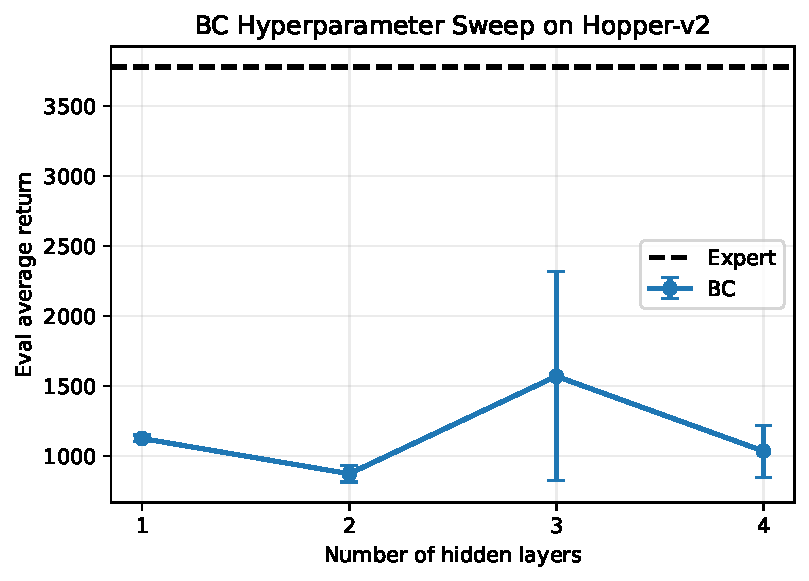
\includegraphics[width=0.65\columnwidth]{bc_layers_sweep.pdf}
  \caption{BC agent's performance vs.\ the number of hidden layers on Hopper-v2. I swept depth because model capacity can affect how well behavior cloning fits the expert action labels, and Hopper-v2 was chosen because the BC baseline had a large gap from expert performance. Other settings were fixed to hidden size 64, learning rate $5\times 10^{-3}$, batch size 1000, train batch size 100, \texttt{eval\_batch\_size}=1000, and 1000 training steps.}
  \label{fig:p4}
\end{figure}

\subsection{Part 5 (0.5 pt)}
Find one robotics paper from the last $\sim$3 years that uses imitation learning (i.e. behavior cloning) as the primary methodology. In a short paragraph (4-5 sentences): (i) cite it, (ii) say what robot task is being cloned and where the expert data comes from and (iii) name a main IL risk from this homework and whether that still applies to the paper's methodology. A few sentences is enough; this is not meant to be an extensive literature review.

Chi et al.~\cite{chi2023diffusionpolicy} propose Diffusion Policy, a visuomotor imitation learning method that represents a robot policy as a conditional denoising diffusion process over action sequences. The cloned tasks are robot manipulation behaviors across simulated and real-world benchmarks, where expert data is provided as demonstration trajectories of observations and actions. The method is still trained in a behavior-cloning style from offline demonstrations, but the diffusion formulation helps model multimodal action distributions and high-dimensional action sequences. A main risk from this homework is compounding error from distribution shift: when the learned policy enters states not well covered by the demonstrations, small action errors can accumulate into poor rollouts. This risk still applies to Diffusion Policy because it is trained from offline demonstrations, although action-sequence prediction and receding-horizon execution can make it more robust than simple one-step BC.


\newpage
\section{DAgger (5 pt)}

\subsection{Part 2 (5 pt)}
\begin{figure}[!h]
  \centering
  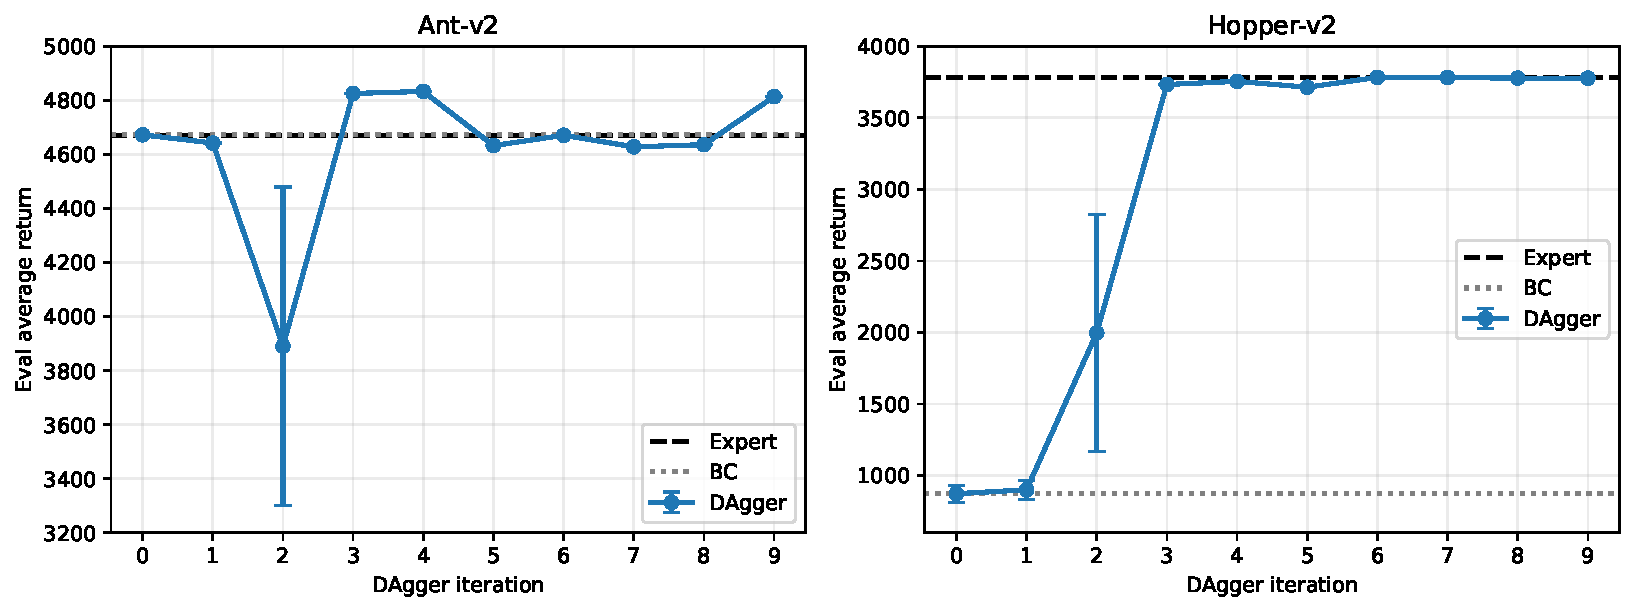
\includegraphics[width=\columnwidth]{dagger_curves.pdf}
  \caption{DAgger learning curves on Ant-v2 and Hopper-v2 over 10 iterations. The dashed lines show expert performance and the dotted lines show the BC baseline. We used a 2-layer MLP with hidden size 64, learning rate $5\times 10^{-3}$, batch size 1000, train batch size 100, \texttt{eval\_batch\_size}=1000, and 1000 policy updates per iteration.}
  \label{fig:p5}
\end{figure}

\begin{thebibliography}{1}

\bibitem{chi2023diffusionpolicy}
Cheng Chi, Zhenjia Xu, Siyuan Feng, Eric Cousineau, Yilun Du, Benjamin Burchfiel, Russ Tedrake, and Shuran Song.
\newblock Diffusion Policy: Visuomotor Policy Learning via Action Diffusion.
\newblock Robotics: Science and Systems (RSS), 2023.

\end{thebibliography}

\end{document}
